\documentclass{report}

\usepackage[utf8]{inputenc}
\usepackage[francais]{babel}
\usepackage[T1]{fontenc}
\usepackage{graphicx}
\usepackage{color}
\usepackage{amsmath}
\usepackage{amssymb}
\usepackage{lmodern}
\usepackage[top=2cm, bottom=2cm, right=2cm, left=2cm]{geometry}
\usepackage{verbatim}

\title{Rapport du projet de graphes}
\author{Baptiste Prunot
\and Amaury Sauvage
\and Raphael Pinto
\and Hugo Ouertani
\and Cyril Vandenbosshe}
\date{\today}


\begin{document}
	\maketitle 
	
	\chapter{Generation des graphes et mode manuel}
		\section{generation des graphes}
			
			\paragraph{\textcolor{blue}{graphe de la carte}}
			Le graphe de la carte est la base sur laquelle vont \^etre g\'en\'er\'es le graphe des zombies, et celui des licornes.
			
			le graphe a la particularit\'e de repr\'esenter une carte avec des cases hexagonales. De ce fait, sa g\'en\'eration a entrain\'e quelques particularit\'es.
			
			Pour expliquer la methode utilis\'ee pour g\'en\'erer le graphe nous nous appuierons sur l'exemple d'une carte de taille 2.
			
			\begin{center}
				\framebox[7cm]{
					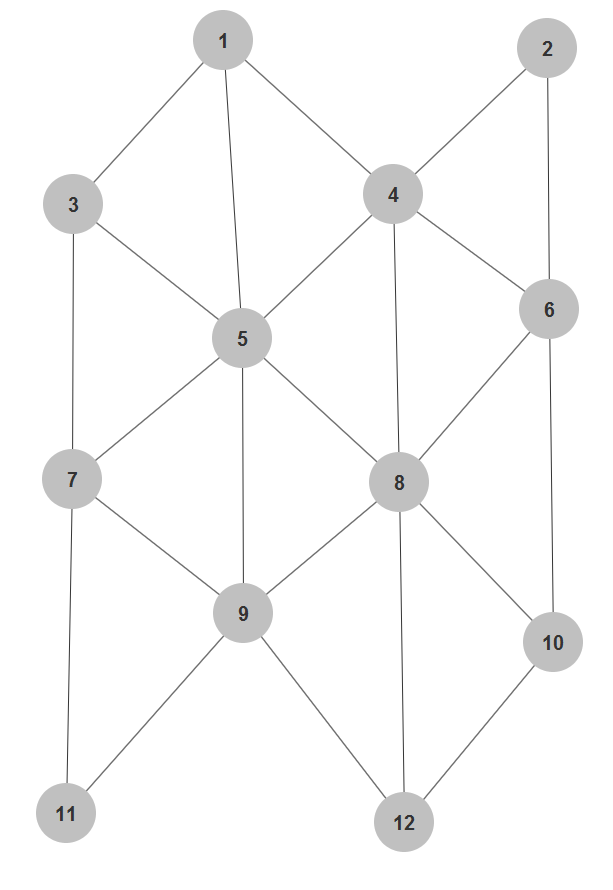
\includegraphics[scale=0.30]{Images/Graphe.png}
				}
			\end{center}
			
			Si nous choisissons le sommet 1, nous remarquons qu'il est li\'e \'a aux sommets suivants :
			
			\itemize{
				\item le sommet 3 ce qui correspond à sommet+2 soit :
				
				
			
				$sommet+tailleGraphe$
				
				\item le sommet 5 ce qui correspond à sommet+4 soit :
				
				
				
				$sommet+tailleGraphe\times2$
				
				\item le sommet 4 ce qui correspond à sommet+3 soit : 
				
				
				
				$sommet+tailleGraphe+1$
				
			}
			
			On pourrait donc conclure que pour générer le graphe il suffirait de lier chaque sommet avec les observations faites ci-dessus. Cependant, bien que lier un sommet à son $sommet+taille\times2$ soit toujours vrai, les deux autres liaisons ne le sont pas forcément. ainsi on distingue deux cas :
			
			
			\itemize{
				\item les lignes paires
				\item les lignes impaires
				}
				
			Lorsque la ligne est paire, un sommet est lié à trois autres sommets :
				
				\itemize{
					\item $sommet+taille\times2$
					\item $sommet+taille$
					\item $sommet+taille-1$
				}
				
			En revanche lorsque la ligne est impaire, les liaisons sont définie de cette manière : 
				
				\itemize{
					\item $sommet+taille\times2$
					\item $sommet+taille$
					\item $sommet+taille+1$
					}
					
			Ces observations aboutissent au code java suivant : 
			\\
			\begin{verbatim}
				public Graphe setGraphe(int taille) {
        Graphe graphe = new Graphe(taille);
        int nbSommet = graphe.getNbSommet();
        int n = this.taille;
        for (int i = 1; i <= nbSommet; i++) { 
            for (int j = 1; j <= n; j++) { 
                int position = j + (n * i) - n;
                if (position + n * 2 <= nbSommet) { 
                    graphe.ajouterArc(position, position + n * 2, 1);

                }
                if (position + n <= nbSommet) {
                    graphe.ajouterArc(position, position + n, 1);
                }

                if (i % 2 != 0) {    
                    if ((position + n + 1 <= nbSommet) && (j < n)) { 
                        graphe.ajouterArc(position, position + n + 1, 1);
                    }
                } else if (position + n - 1 <= nbSommet && (j > 1 && j <= n)) {
                    graphe.ajouterArc(position, position + n - 1, 1);
                }
            }
        }
        return graphe;
    }
			\end{verbatim}
								
			
			
			
			
			
			
			
			
			\paragraph{graphe des licornes}
			\paragraph{graphe des zombies}
		\section{Mode manuel}
			\paragraph{Effacer la coloration}
			\paragraph{couleurs et distances}
			\paragraph{Mise en place de la coloration}
			
			
	\chapter{mode automatique}
		\section{Les races de base}
			\paragraph{\textcolor{blue}{Mouvement des licornes}}
			Le principe ici est de calculer un Dijkstra puis grâce à une fonction on va pouvoir construire un chemin en se basant sur les antécédents de la planète.
			\paragraph{\textcolor{blue}{Mouvement des zombies}}
			Le principe ici est de recalculer un Dijkstra à chaque itération étant donné que le vaisseau des licornes est en mouvement.La fonction permettant de construire un chemin est ici réutilisée.
			\paragraph{\textcolor{blue}{Les shadocks}}
			Le principe ici est de calculer un Dijkstra de la planète Shadock puis de stocker les sommet à 3 ou moins de distances dans un ArrayList.Puis on sélectionne des sommets aléatoirement si le sommet et à moins de 1 de distances qui sera déterminée par un Dijkstra à partir du vaisseau alors celui ci se déplace.
			\paragraph{\textcolor{blue}{Optimisation des gibis}}
			\paragraph{\textcolor{blue}{Navigation suicidaire}}
			Le principe ici est de faire en sorte que le vaisseau licorne ne se jette pas sur le vaisseau des zombies.
			Pour ce faire il suffit de reprendre le principe d'isolation du sommet su soleil.
			Ainsi le vaisseau de licorne n'ira pas sur la case vaisseau zombie en automatique et sera également géré dans le mode manuel
			\paragraph{\textcolor{blue}{Coloniser plusieurs planètes}}
	\setcounter{tocdepth}{4}
	\tableofcontents
\end{document}
